\documentclass[11pt]{article}

\usepackage[margin=1in]{geometry}
\usepackage{booktabs}
\usepackage{amsmath}
\usepackage{hyperref}
\usepackage{graphicx}
\usepackage{float}
\usepackage{subcaption}

\title{EC4308 Project --- Tree-Based Models and Interpretability}
\author{}
\date{}

\begin{document}
\maketitle


\section*{Methodology}

\subsection*{Tree-Based Classifiers}

We fit three tree-based classifiers: a single Decision Tree (DT), Random
Forest (RF), and XGBoost (XGB). RF is the best-performing model reported by
Islam et al.\ (2019). The single Decision Tree serves as the interpretable
building block of RF and provides a lower bound on tree-based performance.
XGBoost, a gradient-boosted tree ensemble, is included as an extension beyond
the original paper to test whether additional model capacity yields gains on
this dataset.

All three models are evaluated using both an 80/20 stratified hold-out split
and 10-fold stratified cross-validation, consistent with the evaluation
protocol in the original paper. We set \texttt{random\_state=42} throughout
to ensure reproducibility. Default hyperparameters are used in the first
instance to match the paper's protocol: RF with 100 trees; a fully-grown
Decision Tree with Gini splits; XGBoost with 100 rounds,
\texttt{max\_depth=6}, and \texttt{learning\_rate=0.1}.

\subsection*{Interpretability}

We assess feature importance at two levels. At the global level, we compute
native Gini importance for RF and total-gain importance for XGBoost. At the
local level, we compute SHAP (SHapley Additive exPlanations) values
(Lundberg and Lee, 2017). SHAP decomposes each individual prediction into
signed additive contributions from each feature and is grounded in
cooperative game theory. In contrast to Gini importance, which returns an
unsigned aggregate score per feature, SHAP values indicate the direction in
which each feature pushes a given prediction and can be aggregated across
samples to produce a global importance ranking with preserved sign
information. SHAP values are computed using the exact \texttt{TreeExplainer}.

\subsection*{Robustness Checks}

Two additional analyses assess whether the results are sensitive to sample
size or hyperparameter choice. First, we construct learning curves by
retraining each model on increasing subsets of the data and recording 10-fold
cross-validated accuracy. Second, we conduct hyperparameter tuning via
\texttt{GridSearchCV} with 10-fold accuracy scoring. The search grids are:

\begin{itemize}
    \item RF: $n_\text{est}\!\in\!\{50,100,200\}$,
    $\text{max\_depth}\!\in\!\{\text{None},5,10,15\}$,
    $\text{min\_samples\_split}\!\in\!\{2,5,10\}$.
    \item DT: $\text{max\_depth}\!\in\!\{\text{None},3,5,7,10\}$,
    $\text{min\_samples\_split}\!\in\!\{2,5,10,20\}$,
    $\text{criterion}\!\in\!\{\text{gini},\text{entropy}\}$.
    \item XGB: $n_\text{est}\!\in\!\{50,100,200\}$,
    $\text{max\_depth}\!\in\!\{3,6,9\}$,
    $\eta\!\in\!\{0.01,0.1,0.2\}$.
\end{itemize}


\section*{Results}

\subsection*{Classification Performance}

Table~\ref{tab:tree-holdout} reports hold-out performance and
Table~\ref{tab:tree-cv} the 10-fold cross-validation results. Random Forest
achieves 98.3\% cross-validated accuracy, closely matching the 97.4\% figure
reported by Islam et al.\ (2019). XGBoost attains the same hold-out accuracy
as RF (99.04\%) but does not exceed it, suggesting that the additional
capacity of gradient boosting does not translate into predictive gains on
this dataset. The single Decision Tree trails the two ensembles by
approximately one percentage point, indicating that the classification
boundary is close to linearly separable. Precision is 1.000 for all three
models; all classification errors are false negatives.

\begin{table}[H]
\centering
\small
\caption{Hold-out (80/20) performance on the test set.}
\label{tab:tree-holdout}
\begin{tabular}{lccccc}
\toprule
Model & Accuracy & Precision & Recall & F1 & AUC \\
\midrule
Decision Tree & 0.9712 & 1.0000 & 0.9531 & 0.9760 & 0.9766 \\
Random Forest & 0.9904 & 1.0000 & 0.9844 & 0.9921 & 1.0000 \\
XGBoost       & 0.9904 & 1.0000 & 0.9844 & 0.9921 & 0.9996 \\
\bottomrule
\end{tabular}
\end{table}

\begin{table}[H]
\centering
\small
\caption{10-fold stratified cross-validation.}
\label{tab:tree-cv}
\begin{tabular}{lcc}
\toprule
Model & Accuracy (mean $\pm$ sd) & AUC (mean $\pm$ sd) \\
\midrule
Decision Tree & $0.9731 \pm 0.0214$ & $0.9725 \pm 0.0222$ \\
Random Forest & $0.9827 \pm 0.0181$ & $0.9991 \pm 0.0016$ \\
XGBoost       & $0.9788 \pm 0.0135$ & $0.9941 \pm 0.0060$ \\
\bottomrule
\end{tabular}
\end{table}

The structure of the fitted Decision Tree is consistent with this finding:
the root split is on \texttt{polyuria}, followed by \texttt{polydipsia} and
\texttt{gender}. These three variables alone account for the majority of
observed partitioning.

\subsection*{Feature Importance}

Table~\ref{tab:importance} reports five complementary importance
metrics for each of the 16 features. Columns 2--4 are impurity-based:
mean decrease in Gini impurity for the Decision Tree and Random Forest,
and total gain for XGBoost. Columns 5--6 are mean $|\text{SHAP}|$ on
the test set under RF and XGBoost, computed with the exact
\texttt{TreeExplainer}. SHAP values for the Decision Tree are omitted:
applied to a single fully-grown tree, they reduce to a deterministic
propagation of that tree's splits and provide no information beyond
the impurity importance already reported in column~2. Absolute
magnitudes are not directly comparable across columns --- the impurity
columns are normalised shares, RF SHAP is in probability units, and
XGBoost SHAP is in log-odds units --- but ordinal rankings are. Rows
are sorted by the average rank across all five columns.

\begin{table}[H]
\centering
\small
\caption{Feature importance under three tree-based models using
impurity-based measures and mean $|\text{SHAP}|$ on the test set.
Rows sorted by average rank across the five columns.}
\label{tab:importance}
\begin{tabular}{lccccc}
\toprule
 & \multicolumn{3}{c}{Impurity} & \multicolumn{2}{c}{Mean $|\text{SHAP}|$} \\
\cmidrule(lr){2-4}\cmidrule(lr){5-6}
Feature & DT & RF & XGB & RF & XGB \\
\midrule
polyuria            & 0.416 & 0.216 & 0.213 & 0.166 & 1.655 \\
polydipsia          & 0.080 & 0.185 & 0.303 & 0.129 & 1.719 \\
gender              & 0.116 & 0.115 & 0.101 & 0.078 & 0.816 \\
age\_scaled         & 0.093 & 0.099 & 0.019 & 0.022 & 0.405 \\
alopecia            & 0.071 & 0.047 & 0.051 & 0.027 & 0.280 \\
sudden\_weight\_loss & 0.026 & 0.055 & 0.026 & 0.038 & 0.313 \\
irritability        & 0.018 & 0.035 & 0.030 & 0.027 & 0.380 \\
delayed\_healing    & 0.038 & 0.033 & 0.046 & 0.012 & 0.148 \\
genital\_thrush     & 0.029 & 0.020 & 0.039 & 0.011 & 0.184 \\
polyphagia          & 0.000 & 0.031 & 0.034 & 0.023 & 0.236 \\
itching             & 0.003 & 0.030 & 0.033 & 0.025 & 0.361 \\
partial\_paresis    & 0.019 & 0.044 & 0.010 & 0.029 & 0.105 \\
visual\_blurring    & 0.025 & 0.026 & 0.022 & 0.015 & 0.073 \\
muscle\_stiffness   & 0.049 & 0.023 & 0.018 & 0.009 & 0.098 \\
obesity             & 0.018 & 0.018 & 0.036 & 0.005 & 0.081 \\
weakness            & 0.000 & 0.021 & 0.019 & 0.011 & 0.052 \\
\bottomrule
\end{tabular}
\end{table}

The five metrics produce a broadly consistent ranking. All agree on
the top three features (\texttt{polyuria}, \texttt{polydipsia},
\texttt{gender}), which account for 61\% of DT's Gini reduction, 52\%
of RF's, 62\% of XGBoost's total gain, and approximately 55\% of total
mean $|\text{SHAP}|$ under both ensembles --- consistent with the
clinical literature identifying excessive urination and thirst as
primary early indicators of diabetes mellitus. The bottom of the
ranking is likewise stable: \texttt{obesity}, \texttt{weakness},
\texttt{muscle\_stiffness}, and \texttt{visual\_blurring} appear in the
lowest quartile under every metric. The convergence between the
impurity-based and SHAP-based measures lends robustness to the ranking:
it is not an artefact of the well-known bias of Gini importance toward
high-cardinality variables (Strobl et al., 2007).

Two cross-model divergences are nevertheless worth noting. First, the
single Decision Tree concentrates 41.6\% of its total impurity
reduction on \texttt{polyuria}, far more than either ensemble --- a
reflection of its reliance on a single dominant root split, whereas
bagging in RF and residual-fitting in XGBoost spread importance more
evenly. Second, \texttt{age\_scaled} is meaningfully weighted by DT
(0.093) and RF (0.099) but largely discarded by XGBoost (0.019), which
instead allocates its residual capacity to binary symptoms once the
dominant splits have been established. Because the five metrics
otherwise agree, the ranking in Table~\ref{tab:importance} can be
regarded as a well-corroborated summary of feature relevance. The
additional value of SHAP over the impurity columns is therefore not a
different ranking, but the directional and sample-level information
shown in Figure~\ref{fig:shap}, which neither Gini nor gain can
provide.

The SHAP beeswarm plots for RF and XGBoost are shown in
Figure~\ref{fig:shap}. Both models exhibit substantially similar attribution
patterns, reinforcing the consistency of the ranking obtained from Gini and
gain importance. Three patterns not captured by Gini importance are
apparent. First, presence of polyuria and polydipsia produces consistently
positive SHAP values while absence produces consistently negative values,
confirming the expected clinical direction. Second, \texttt{gender} exhibits
sign asymmetry: with the encoding Male~$=1$, male observations contribute
negatively to predicted diabetes probability. This reflects the composition
of the Sylhet hospital cohort, in which positive cases are disproportionately
female; the direction is therefore sample-specific rather than a general
clinical property. Third, \texttt{itching} contributes a small negative
effect. The raw itching rate is 49.5\% among negative cases and 48.1\%
among positive cases (correlation $=-0.013$), and the models correspondingly
assign itching a weak inverse association with the target.

\begin{figure}[H]
\centering
\begin{subfigure}[t]{0.49\textwidth}
\centering
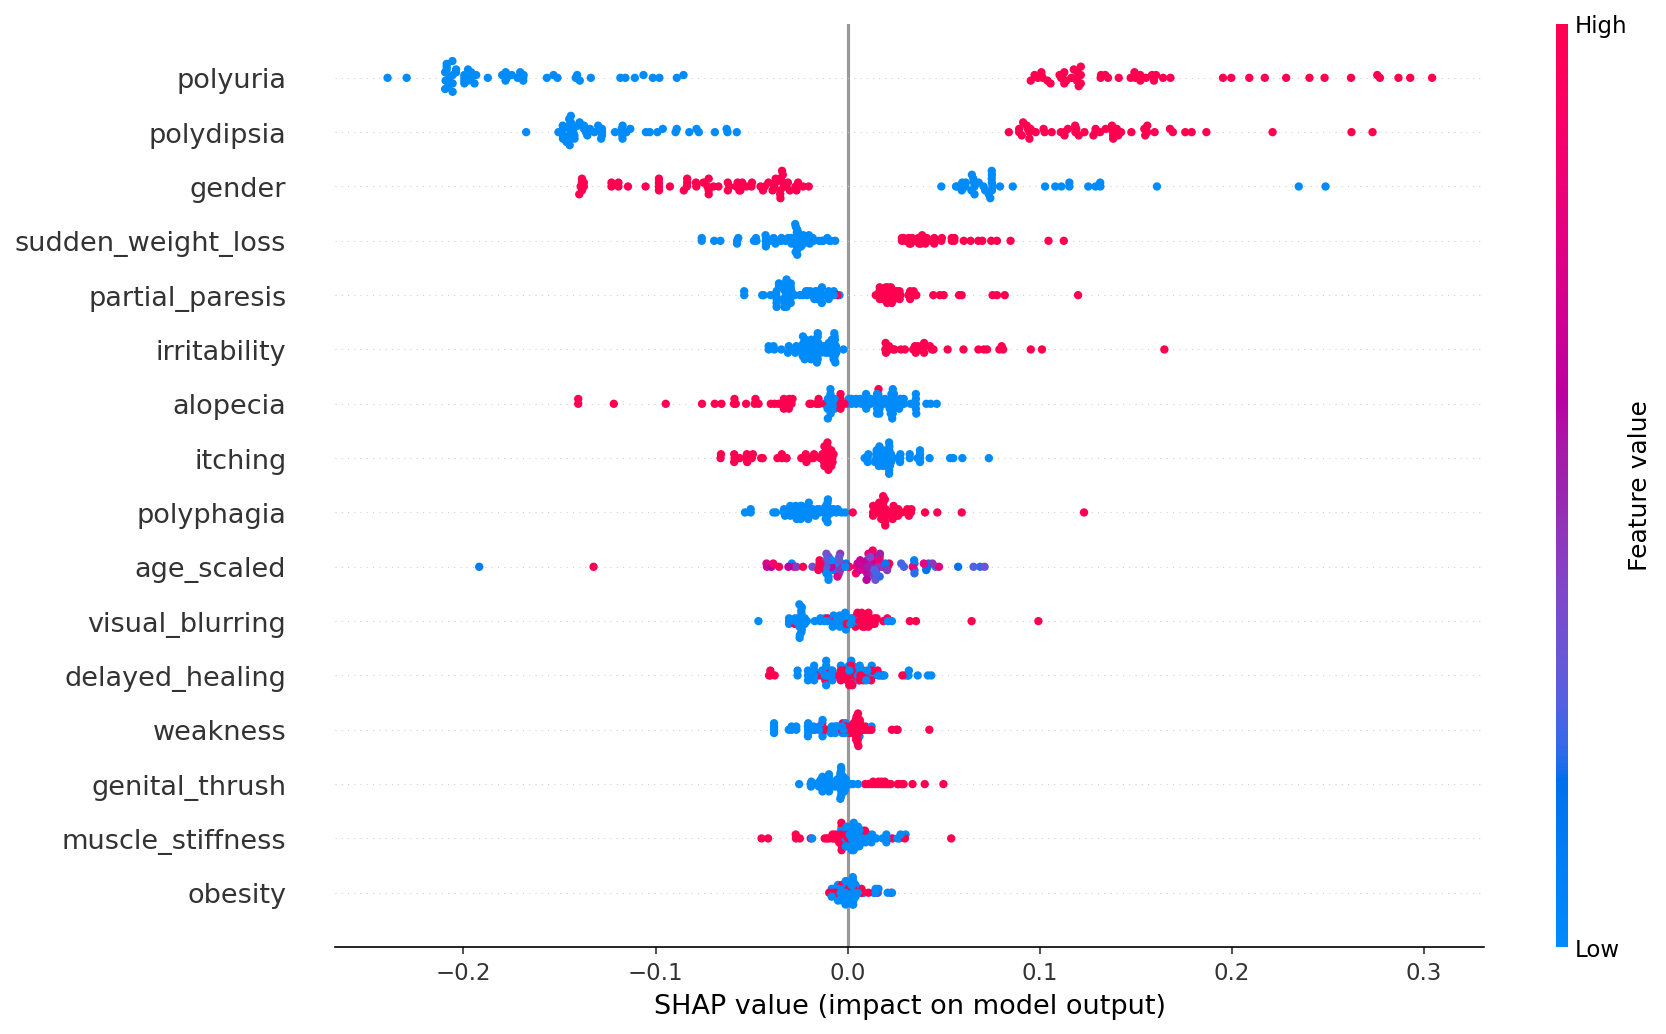
\includegraphics[width=\textwidth]{figures/shap_rf_summary.png}
\caption{Random Forest}
\label{fig:shap-rf}
\end{subfigure}
\hfill
\begin{subfigure}[t]{0.49\textwidth}
\centering
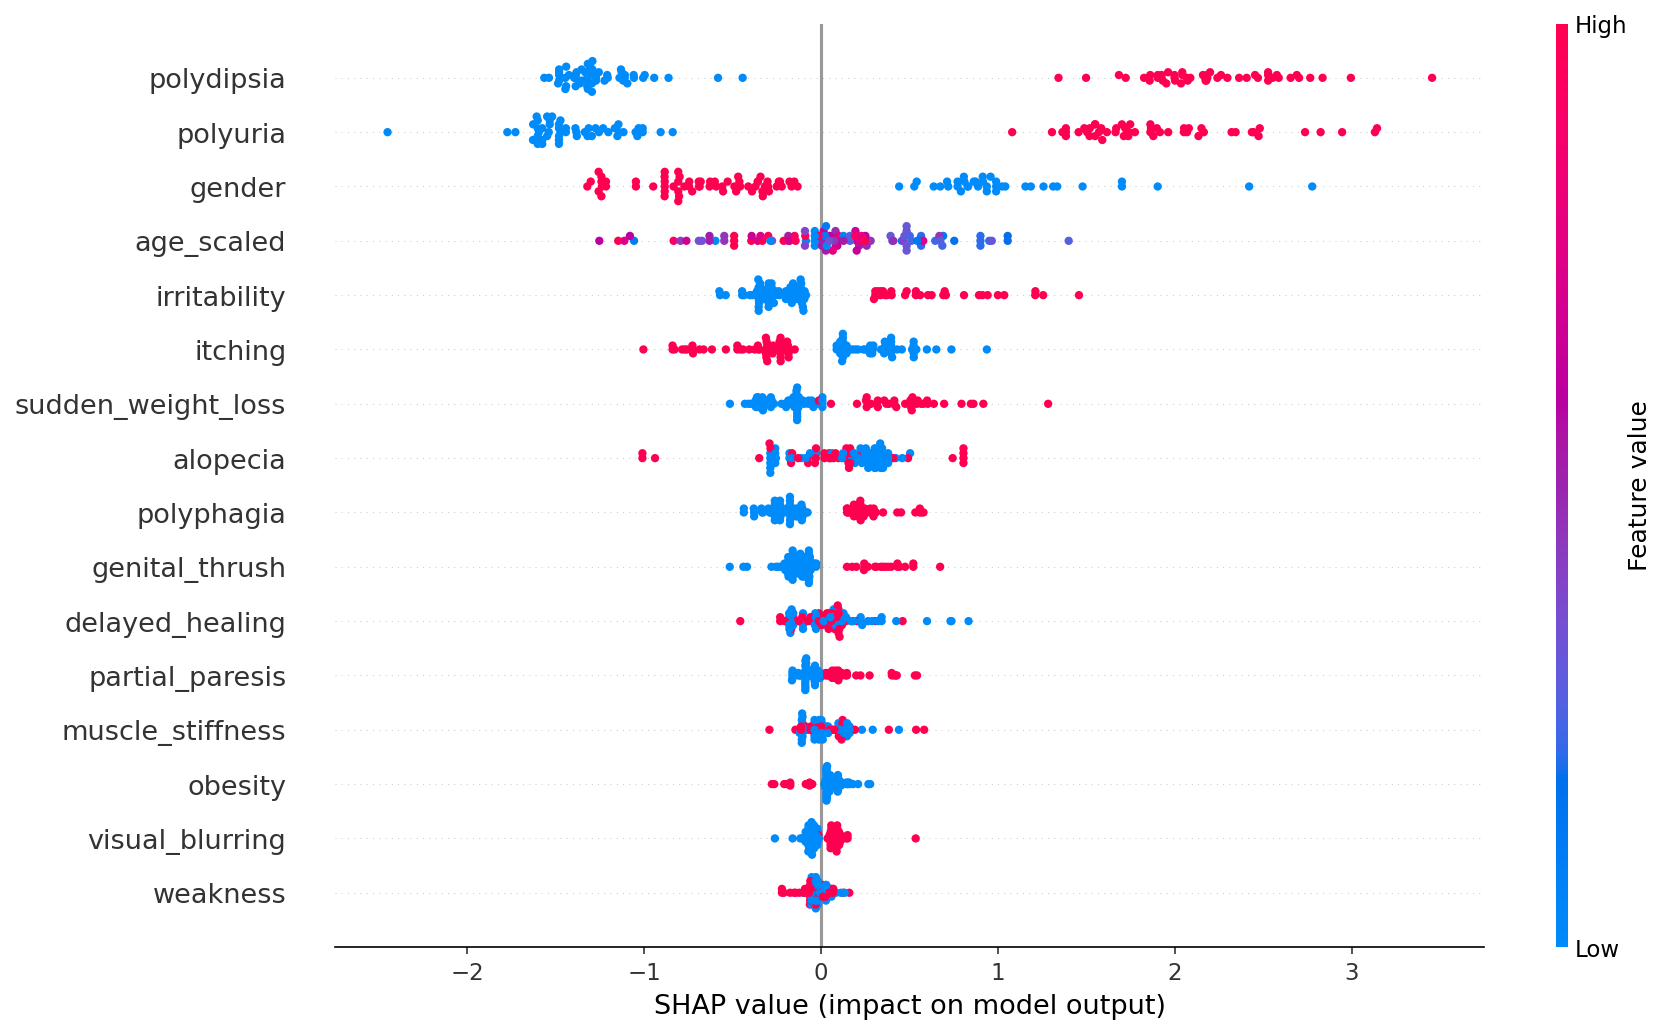
\includegraphics[width=\textwidth]{figures/shap_xgb_summary.png}
\caption{XGBoost}
\label{fig:shap-xgb}
\end{subfigure}
\caption{SHAP beeswarm plots. Each point represents a test observation;
horizontal position denotes SHAP value for the positive class, and colour
denotes the underlying feature value (red = high, blue = low).}
\label{fig:shap}
\end{figure}

\subsection*{Robustness}

All three models attain above 95\% cross-validated accuracy once the training
set exceeds approximately 250 observations, and the gap between training and
validation accuracy remains small throughout (Figure~\ref{fig:learning}). The
absence of a widening gap is inconsistent with overfitting and indicates
that the class-separating signal is strong relative to the sample size.

\begin{figure}[H]
\centering
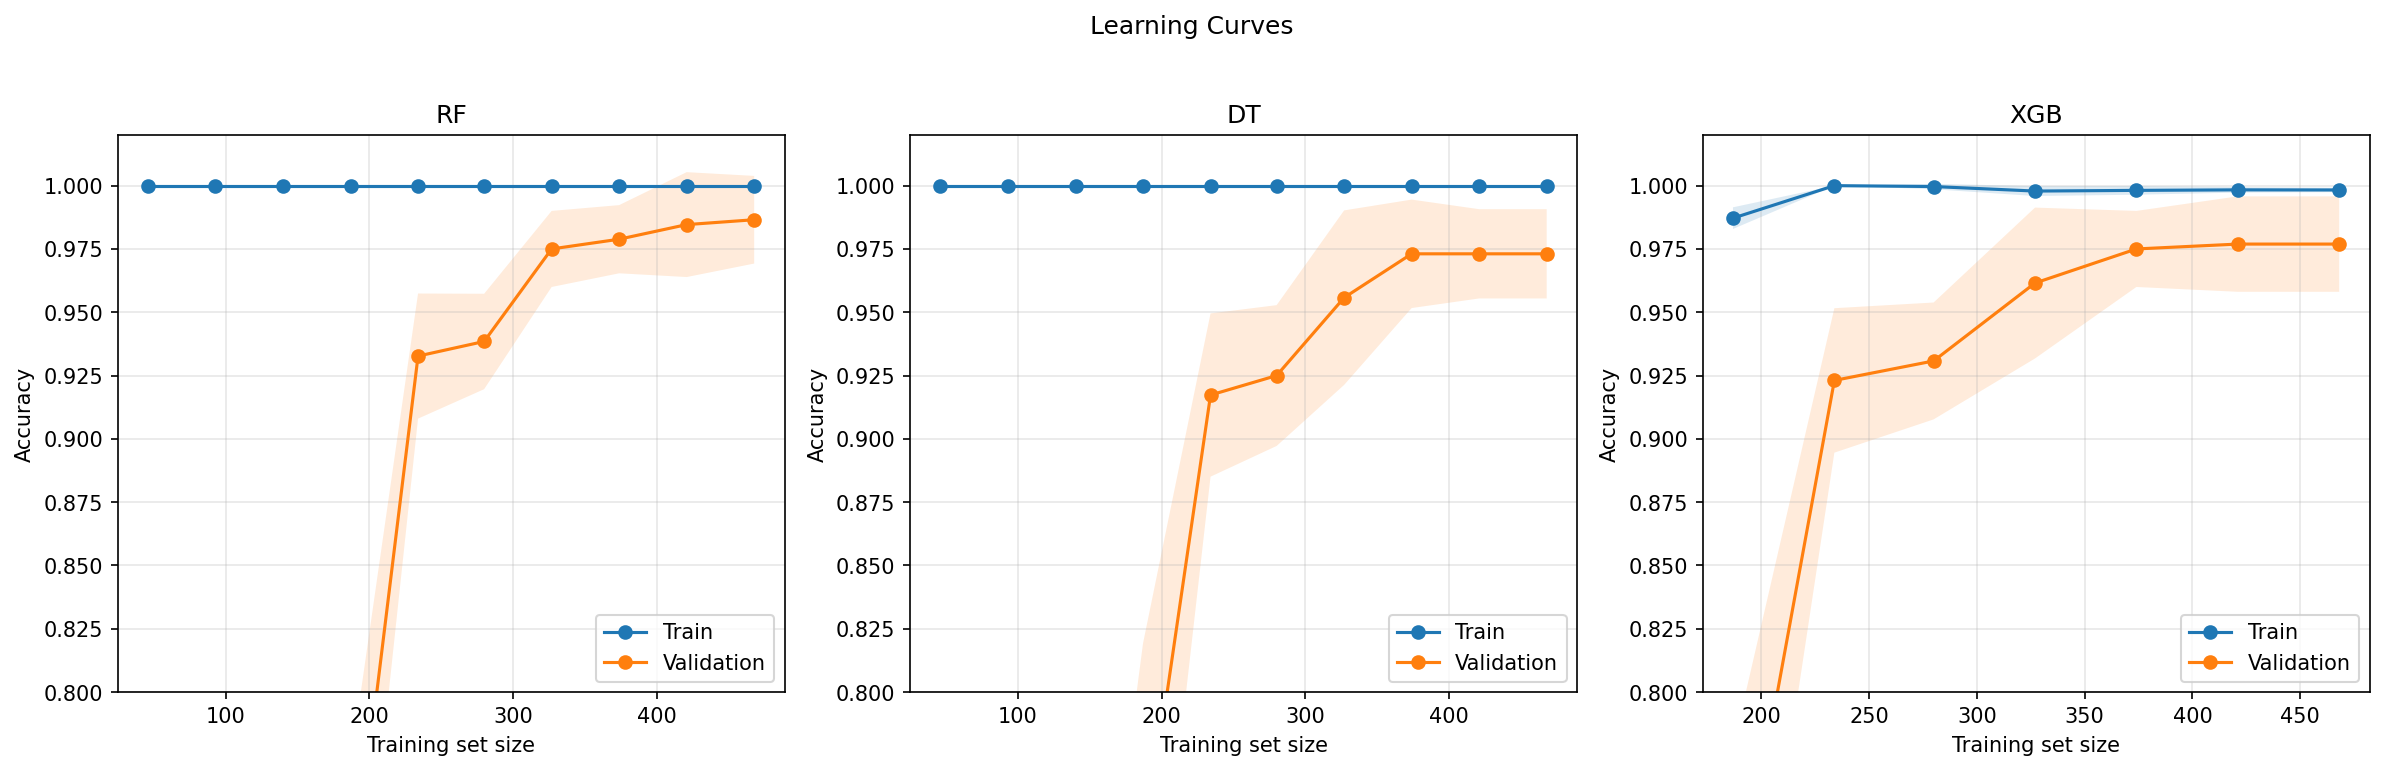
\includegraphics[width=\textwidth]{figures/learning_curves.png}
\caption{Learning curves for RF, DT, and XGBoost. Shaded regions show one
standard deviation of 10-fold cross-validation scores.}
\label{fig:learning}
\end{figure}

Table~\ref{tab:tuning} summarises the hyperparameter tuning results. Tuning
leaves RF unchanged, improves DT by 0.96 percentage points, and marginally
degrades XGBoost (best grid point: \texttt{max\_depth=3},
\texttt{learning\_rate=0.2}, \texttt{n\_estimators=200}). The absence of
systematic gains is consistent with the learning-curve evidence: predictive
performance on this dataset is bounded by the available signal rather than
by model capacity.

\begin{table}[H]
\centering
\small
\caption{Default vs.\ tuned hold-out accuracy.}
\label{tab:tuning}
\begin{tabular}{lccc}
\toprule
Model & Default & Tuned & $\Delta$ \\
\midrule
RF  & 0.9904 & 0.9904 & $+0.0000$ \\
DT  & 0.9712 & 0.9808 & $+0.0096$ \\
XGB & 0.9904 & 0.9808 & $-0.0096$ \\
\bottomrule
\end{tabular}
\end{table}


\section*{Discussion}

The tree-based replication corroborates the headline finding of Islam et
al.\ (2019): Random Forest achieves near-ceiling accuracy on the early-stage
diabetes dataset. Extending the model set to include a single Decision Tree
and XGBoost demonstrates that neither additional ensembling beyond RF nor
gradient boosting yields systematic gains on this data. The combination of
saturating learning curves and null tuning results implies that performance
is bounded by the data rather than by model flexibility.

The SHAP analysis complements the Recursive Feature Elimination results by
providing a directional, sample-level account of feature contribution.
Gini, SHAP, and RFE converge on a consistent top-four ranking (polyuria,
polydipsia, gender, age\_scaled) but diverge in the tail: RFE drops
\texttt{weakness} and \texttt{alopecia} from its optimal subset under
XGBoost, whereas SHAP retains small but non-zero contributions from these
variables. This divergence is expected, as the two methods answer different
questions: RFE identifies the minimal sufficient feature set for prediction,
while SHAP attributes credit across all features used by the fitted model.
Taken together, the two analyses produce a more robust feature ordering
than either in isolation.

A limitation made transparent by the learning curves and the tuning
experiment is the nature of the source data. The dataset consists of 520
patients recruited at a specialty diabetes clinic, and symptom prevalence
is therefore conditional on presentation at such a clinic. On this sample,
any reasonable tree-based classifier approaches 99\% accuracy. The more
informative scientific question is therefore which features carry the
predictive signal, rather than which algorithm is optimal --- a question
the interpretability analysis is designed to address. Validation of these
findings on a general-population screening dataset, where the symptom prior
differs substantially, is a natural direction for future work.


\section*{References}

\begin{itemize}
    \item Islam, M.~F., Ferdousi, R., Rahman, S., \& Bushra, H.~Y. (2019).
    Likelihood prediction of diabetes at early stage using data mining
    techniques. \textit{Computer Vision and Machine Intelligence in Medical
    Image Analysis} (ISCMM 2019), Springer, 113--125.
    \item Lundberg, S.~M., \& Lee, S.-I. (2017). A unified approach to
    interpreting model predictions. \textit{Advances in Neural Information
    Processing Systems} 30 (NeurIPS).
    \item Strobl, C., Boulesteix, A.-L., Zeileis, A., \& Hothorn, T. (2007).
    Bias in random forest variable importance measures: illustrations,
    sources and a solution. \textit{BMC Bioinformatics}, 8(1), 25.
\end{itemize}

\end{document}
